\subsection{Presentation Layer}
\begin{figure}[H]
    \centering
    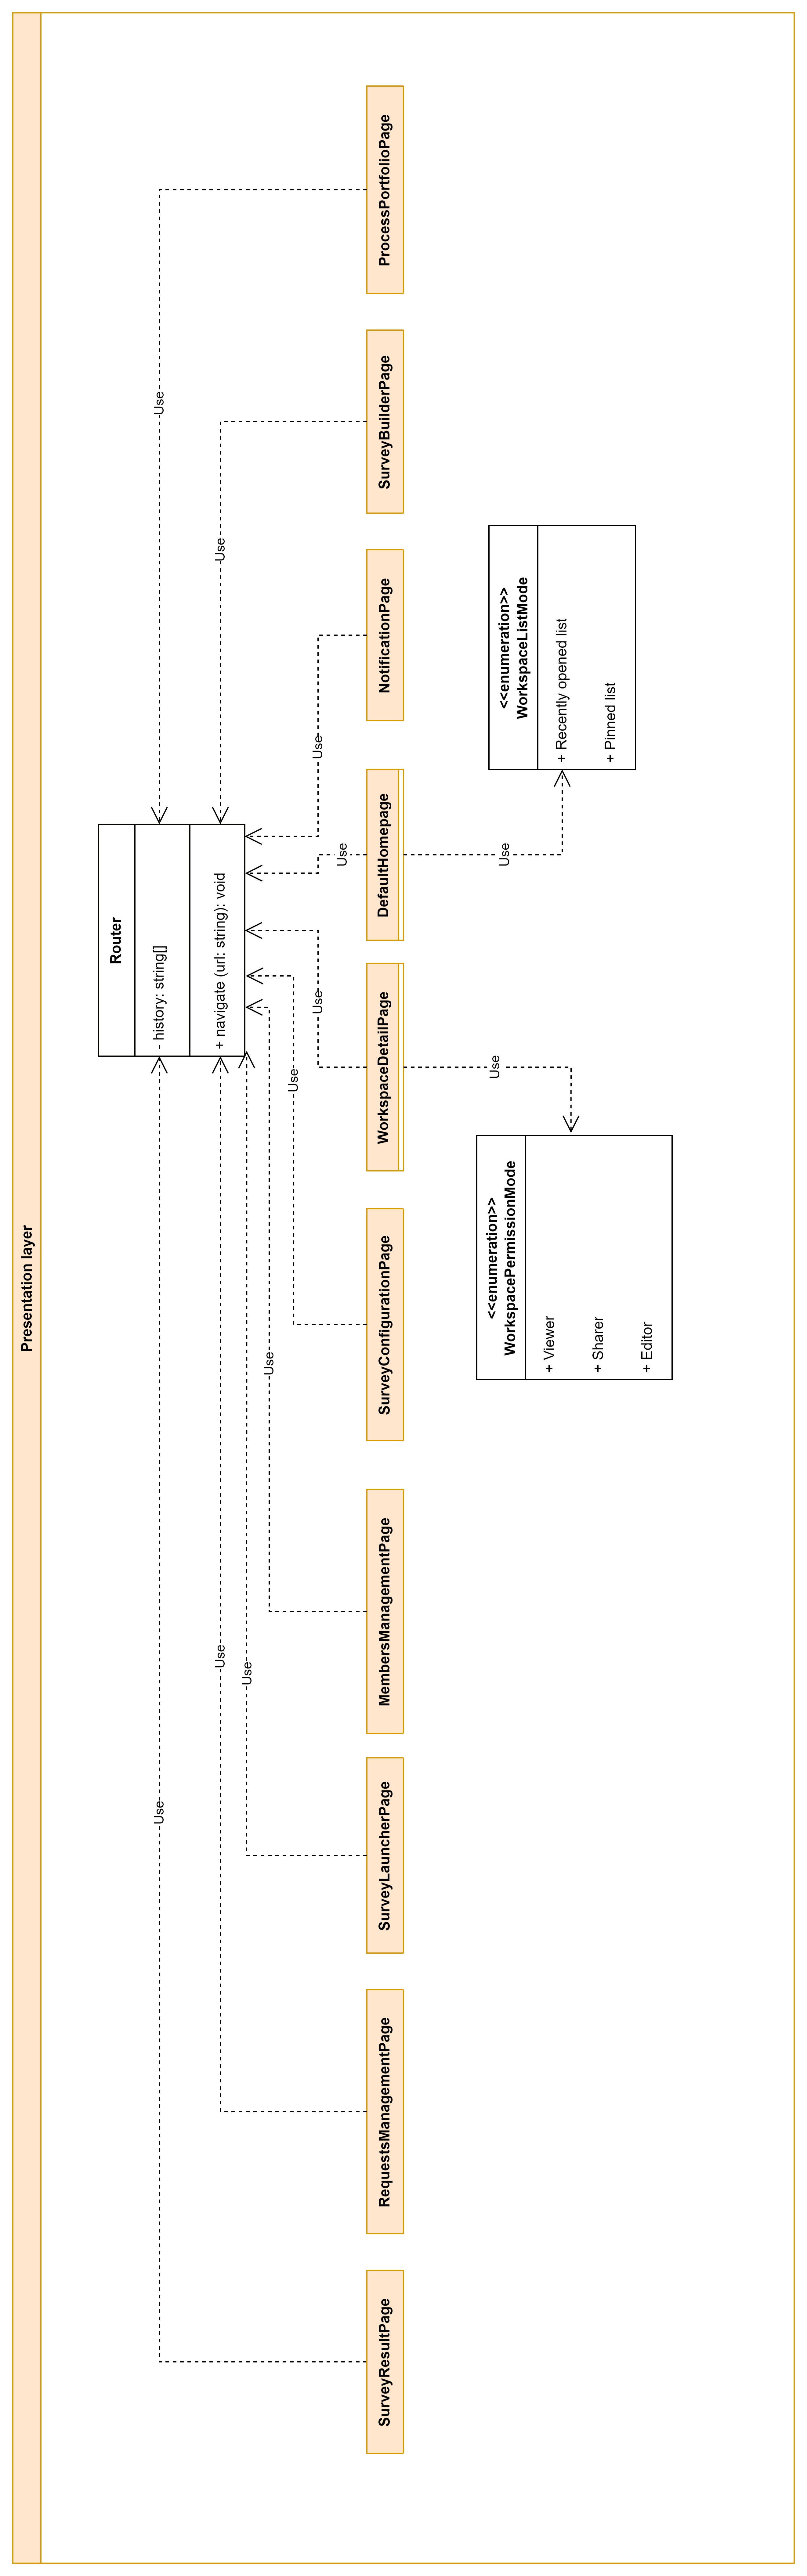
\includegraphics[ height = 0.8\textheight]{Content/Phân tích và thiết kế hệ thống/documents/Sơ đồ lớp/images/Collapsed layer/collapsedPresentationLayer.png}
    \vspace{0.5cm}
    \caption{Tổng quan Presentation Layer}
    \label{fig:Tổng quan Presentation layer}
\end{figure}
Tầng Presentation biểu diễn những giao diện được hiện thực, nó sẽ bao gồm cả những trạng thái (mode) của giao diện cũng như những hàm hiện thực chức năng logic của giao diện tương ứng.
Chi tiết cụ thể hơn sẽ được trình bày trong phần dưới theo từng class được hiện thực.

\begin{figure}[H]
    \centering
    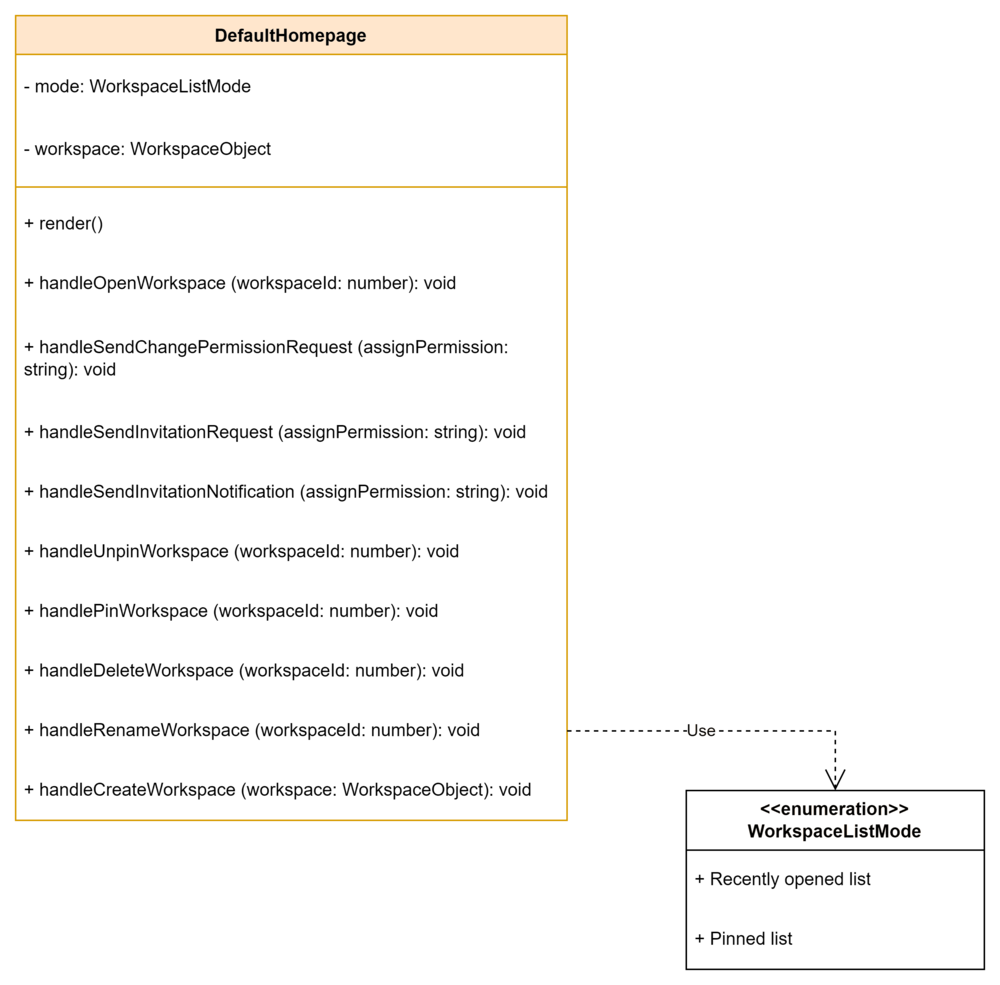
\includegraphics[ width = 0.5\linewidth]{Content/Phân tích và thiết kế hệ thống/documents/Sơ đồ lớp/images/Presentation layer/defaultWorkspacePage.png}
    \vspace{0.5cm}
    \caption{Class DefaultHomepage trong Presentation layer}
    \label{fig:Class Default homepage trong Presentation layer}
\end{figure}
Ở giao diện mặc định khi người dùng được chuyển hướng tới sau khi hoàn tất thủ tục xác thực với hệ thống, chúng ta sẽ tập trung vào những chức năng liên quan tới việc hiển thị và tương tác với workspace mà người dùng tham gia (create, open, pin, delete, rename). Những chức năng đáng chú ý là nhóm chức năng gửi lời mời vào workspace/gửi yêu cầu mời người dùng khác vào workspace, nhóm chức năng này được xử lý real-time (thời gian thực) để nhận và hiển thị dữ liệu ở những giao diện khác. Giao diện sẽ có hai hình thức hiển thị danh sách workspace là theo thời gian mở workspace gần nhất - "Recently opened workspace" và những workspace được người dùng ghim thủ công - "Pinned workspace".

\begin{figure}[H]
    \centering
    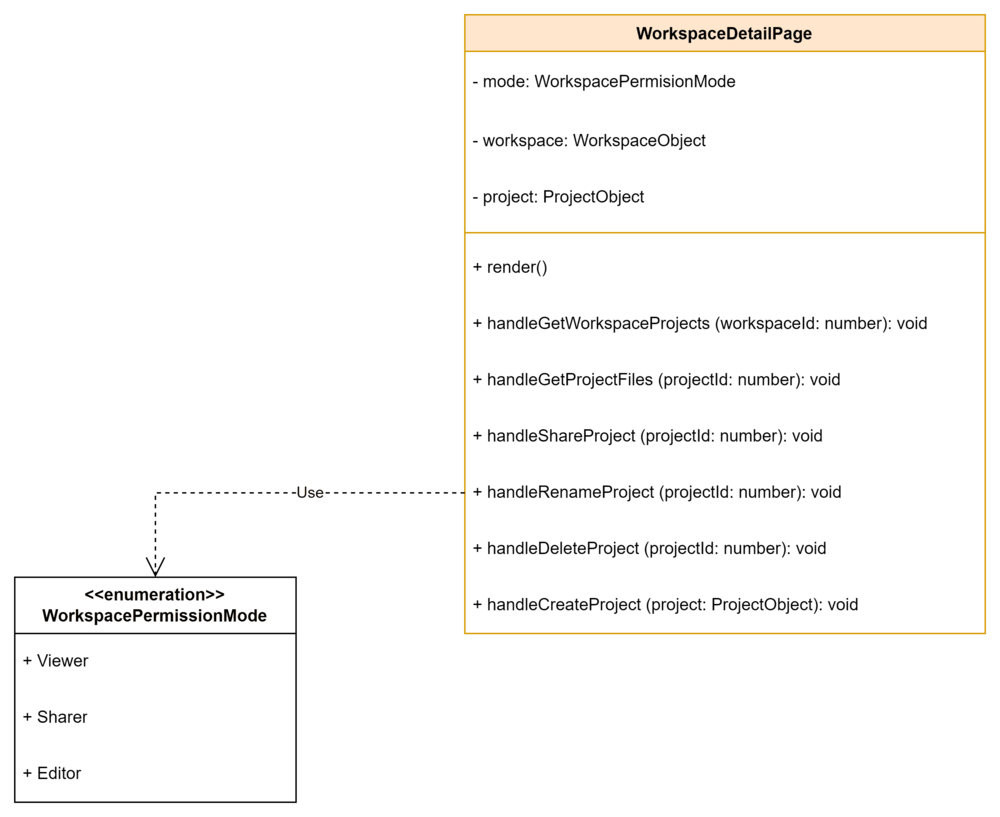
\includegraphics[ width = 0.5\linewidth]{Content/Phân tích và thiết kế hệ thống/documents/Sơ đồ lớp/images/Presentation layer/workspaceDetailPage.png}
    \vspace{0.5cm}
    \caption{Class WorkspaceDetailPage trong Presentation layer}
    \label{fig:Class WorkspaceDetailPage trong Presentation layer}
\end{figure}
Người dùng sẽ được chuyển hướng tới giao diện hiển thị nội dung bên trong workspace khi sử dụng chức năng "Open workspace" hoặc chọn item workspace tương ứng, nội dung bên trong workspace sẽ được hiển thị dưới dạng danh sách những project có bên trong workspace. Mỗi project sẽ là bao gồm nhiều process/version của process và document bên trong. Người dùng sẽ được phân quyền hạn khi tham gia vào workspace: viewer, sharer và editor.

\begin{figure}[H]
    \centering
    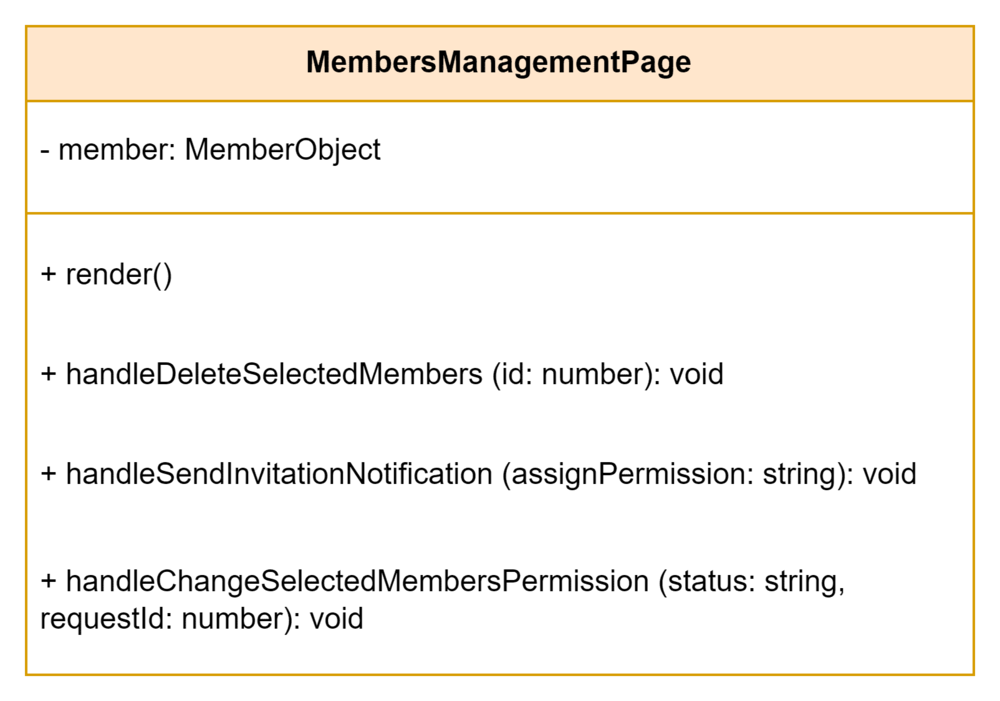
\includegraphics[ width = 0.5\linewidth]{Content/Phân tích và thiết kế hệ thống/documents/Sơ đồ lớp/images/Presentation layer/membersManagementPage.png}
    \vspace{0.5cm}
    \caption{Class MemberManagementPage trong Presentation layer}
    \label{fig:Class MemberManagementPage trong Presentation layer}
\end{figure}
Giao diện quản lý thành viên trong workspace là mục mặc định được điều hướng khi người sở hữu workspace chuyển hướng tới giao diện quản lý. Class này sẽ tập trung hiện thực những chức năng liên quan tới thêm/xóa thành viên trong workspace và điều chỉnh quyền hạn của thành viên tương ứng trong workspace. Ngoài ra còn có chức năng gửi lời mời vào workspace cho người dùng khác, chức năng này cũng sẽ được xử lý real-time để hiển thị dữ liệu ở giao diện thông báo cá nhân khi người dùng khác nhận được lời mời.

\begin{figure}[H]
    \centering
    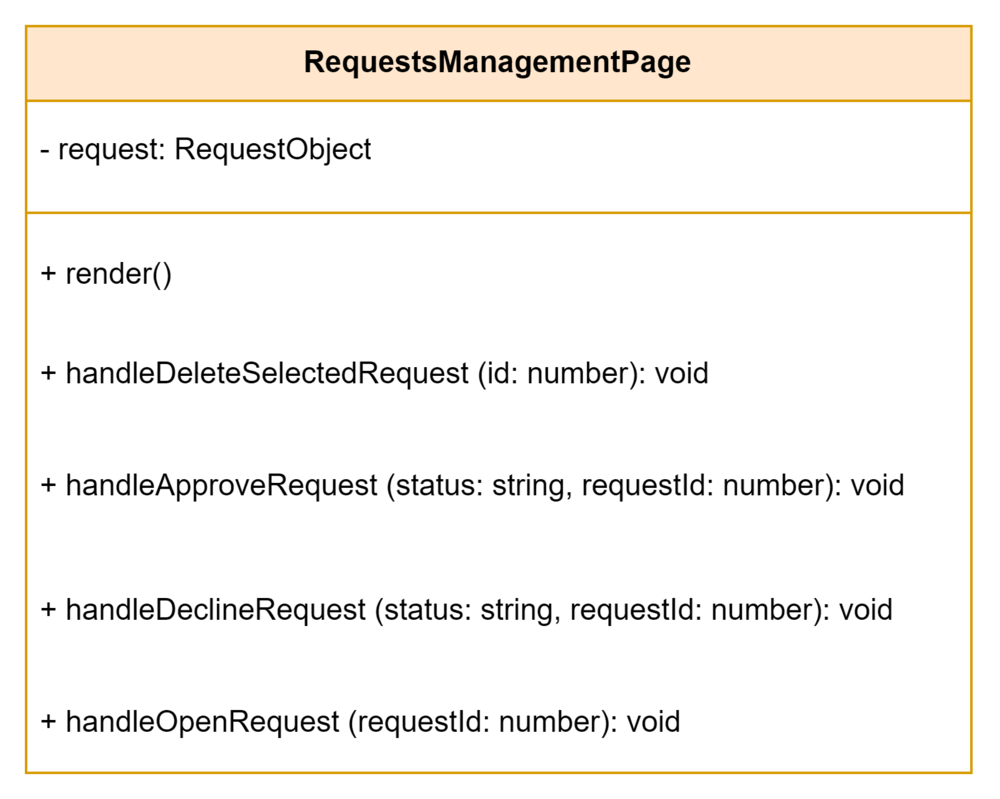
\includegraphics[ width = 0.5\linewidth]{Content/Phân tích và thiết kế hệ thống/documents/Sơ đồ lớp/images/Presentation layer/requestManagementPage.png}
    \vspace{0.5cm}
    \caption{Class RequestManagementPage trong Presentation layer}
    \label{fig:Class RequestManagementPage trong Presentation layer}
\end{figure}
Giao diện quản lý yêu cầu sẽ hiển thị những yêu cầu nhận được từ thành viên bên trong workspace. Những yêu cầu này sẽ được hiển thị dưới dạng danh sách và được phân loại theo loại yêu cầu và trạng thái xử lý của chúng (pending - chờ xử lý, approved - đồng ý hay declined - từ chối).

\begin{figure}[H]
    \centering
    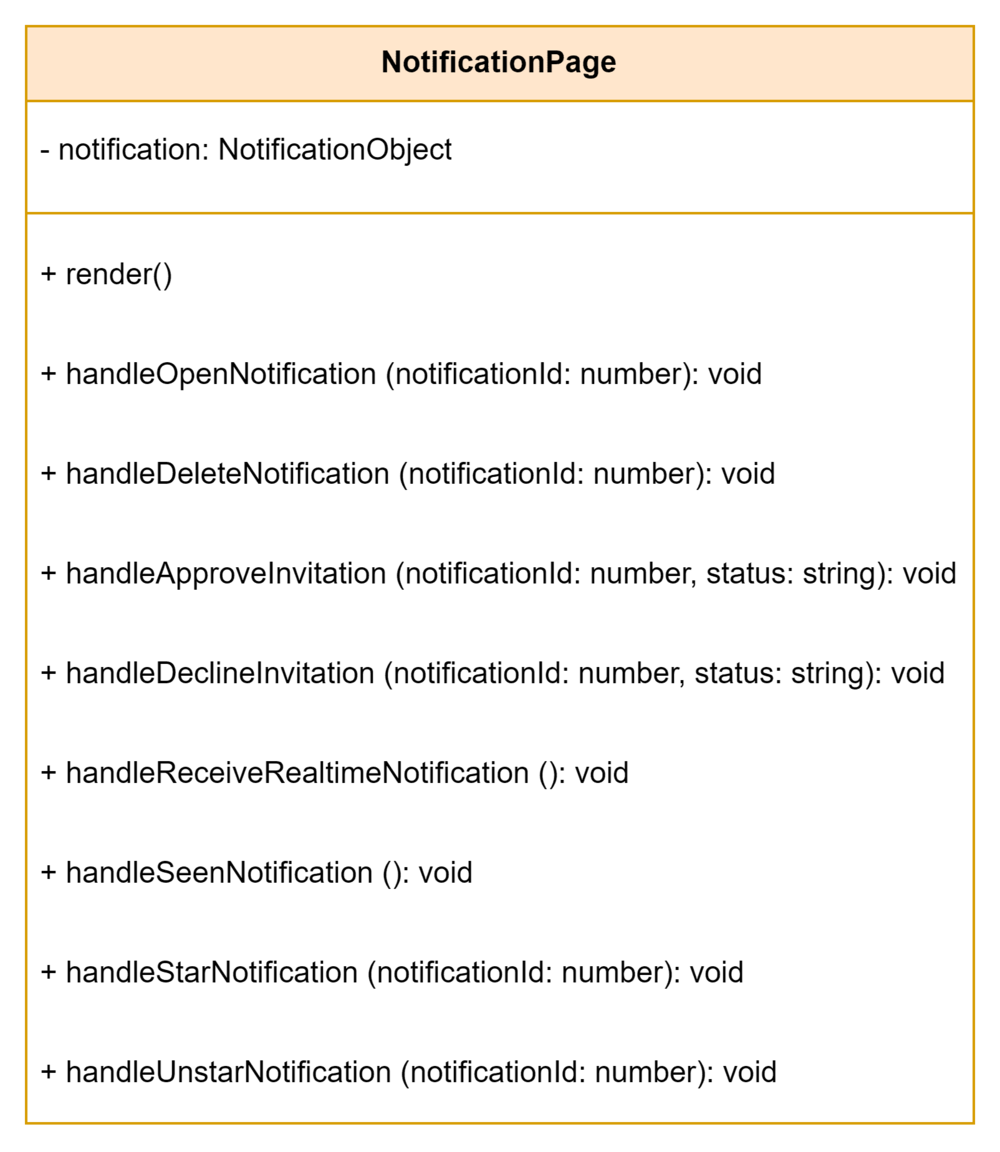
\includegraphics[ width = 0.4\linewidth]{Content/Phân tích và thiết kế hệ thống/documents/Sơ đồ lớp/images/Presentation layer/notificationPage.png}
    \vspace{0.5cm}
    \caption{Class NotificationPage trong Presentation layer}
    \label{fig:Class NotificationPage trong Presentation layer}
\end{figure}
Giao diện thông báo cá nhân là giao diện phụ trách việc hiển thị và giúp người dùng phản hồi những thông báo gửi đến họ. Sẽ có nhiều loại thông báo nhưng trong đó sẽ có thông báo yêu cầu xác nhận từ người dùng (lời mời vào workspace của thành viên trong workspace), hệ thống còn ghi nhận những thông báo đã được đọc và trạng thái của chúng để giúp người dùng có trải nghiệm tốt hơn khi truy xuất những thông báo cần xử lý.

\begin{figure}[H]
    \centering
    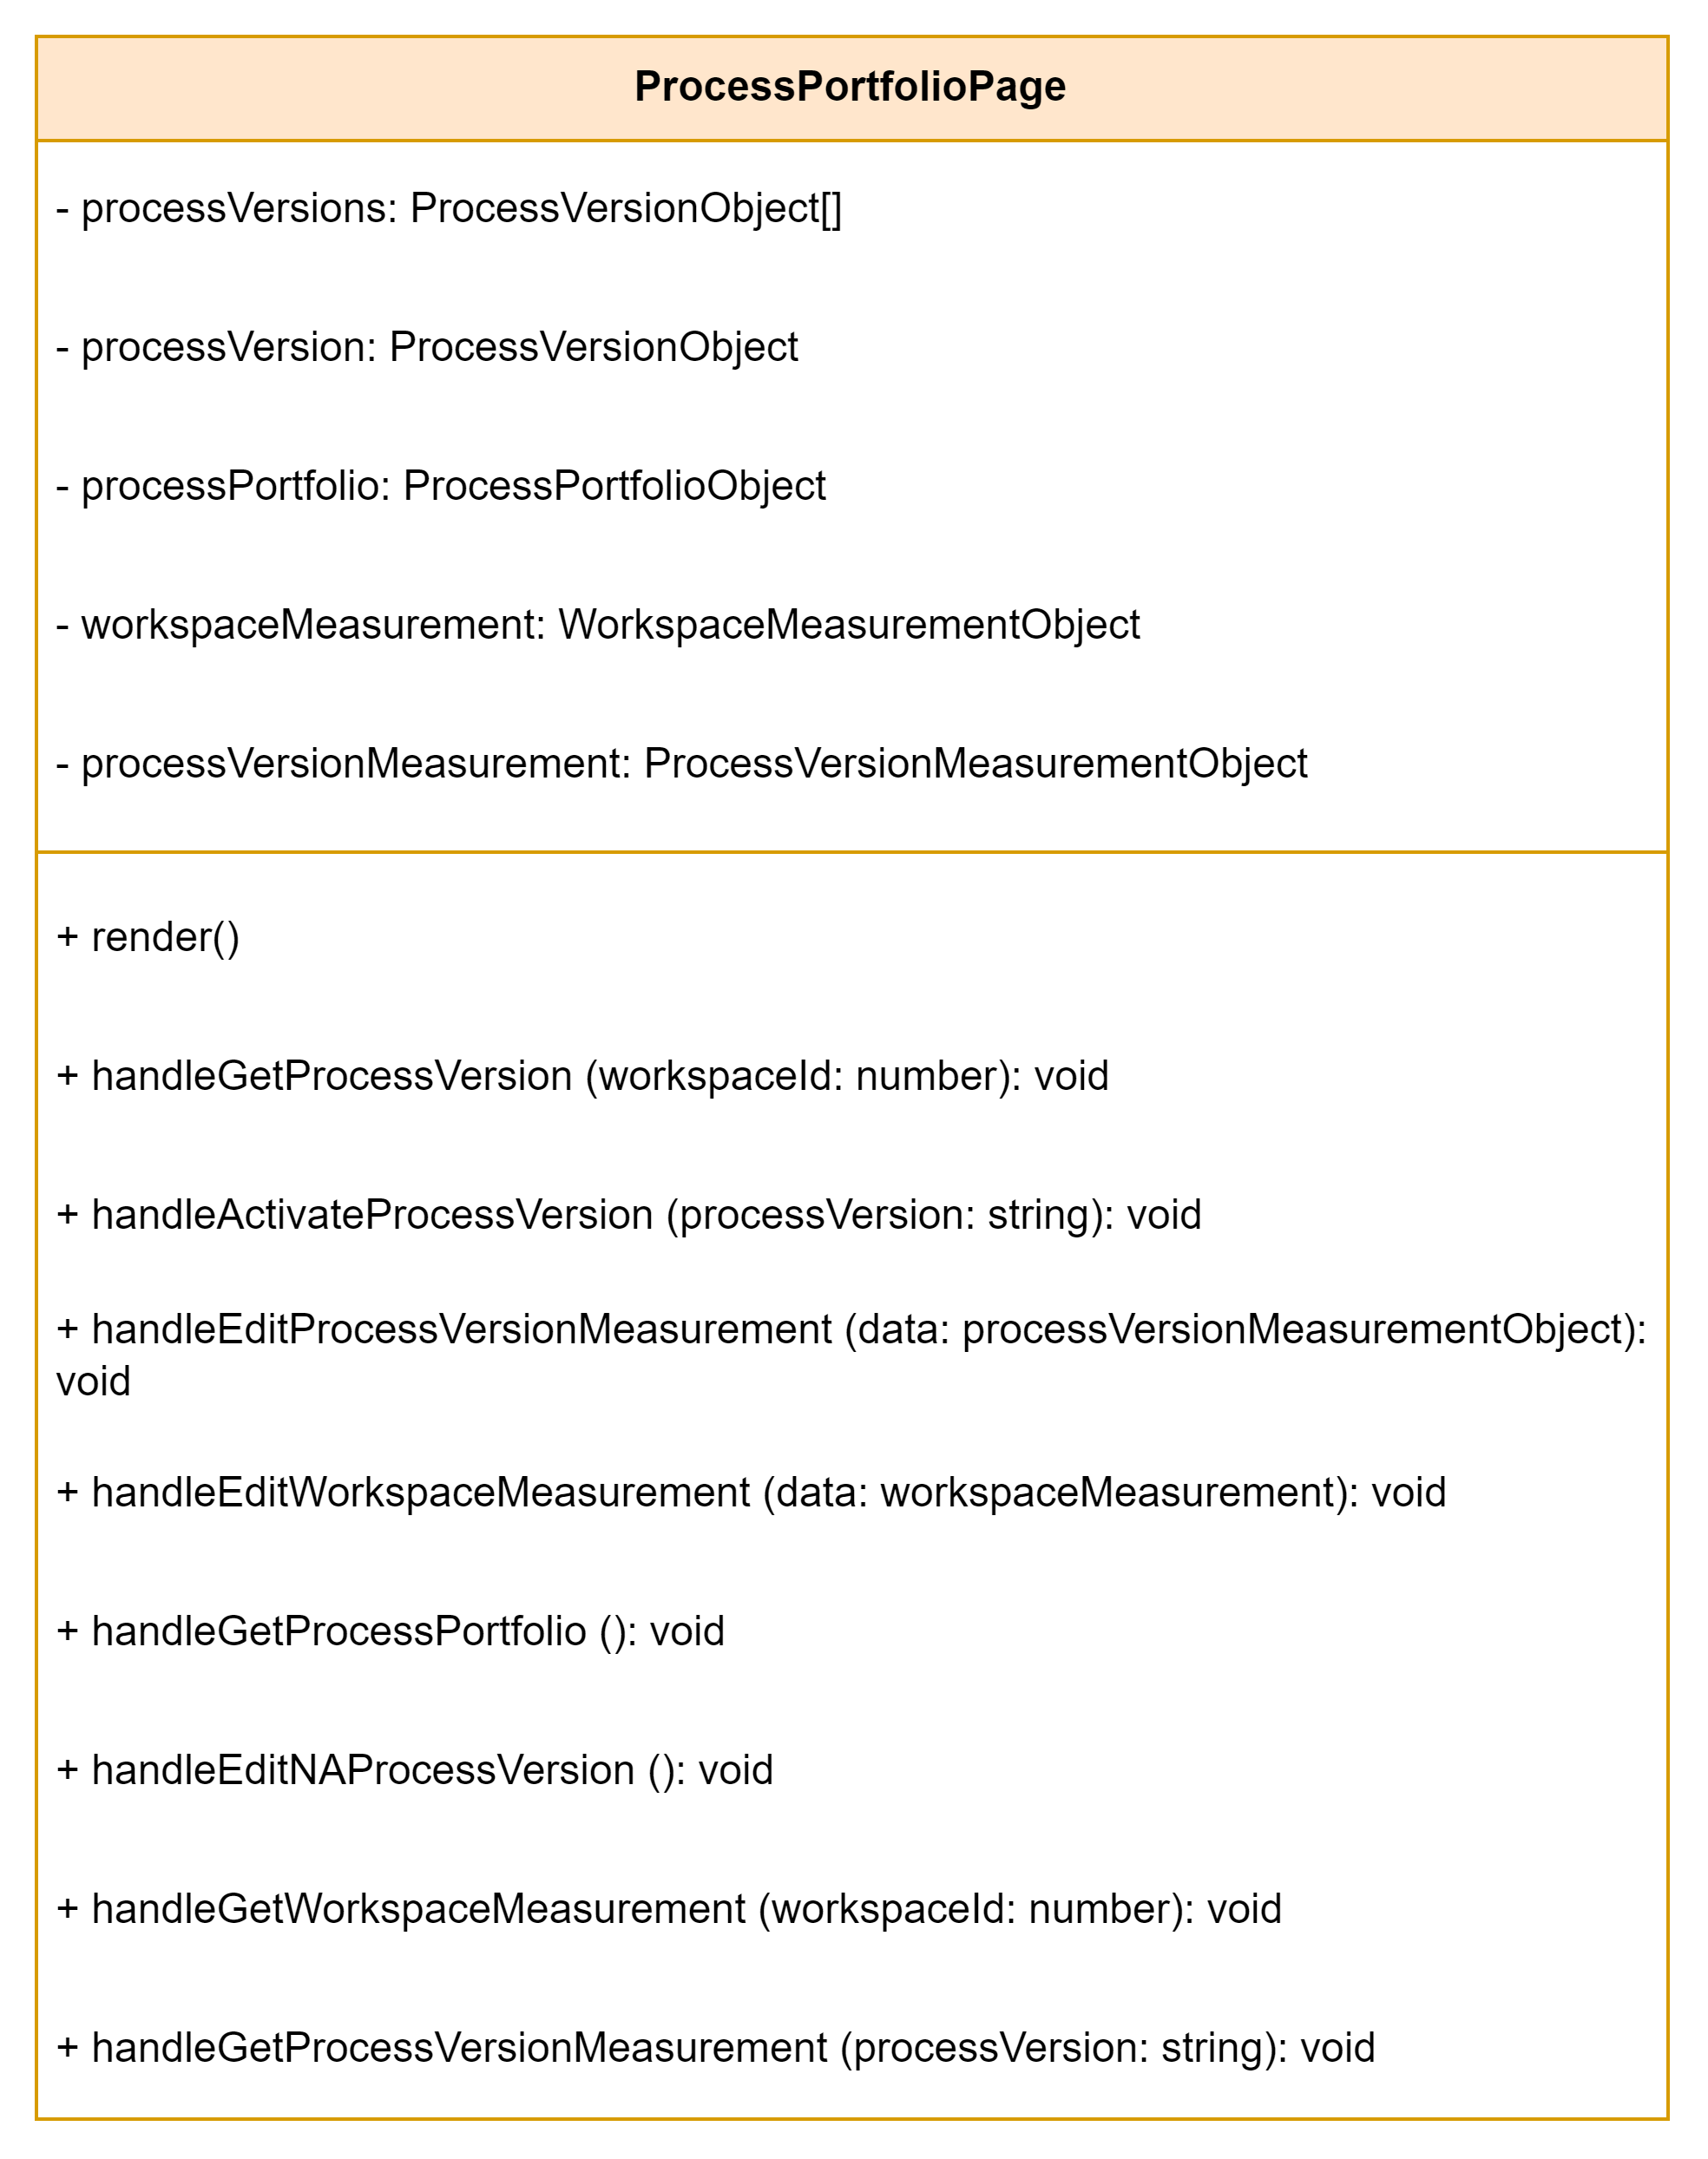
\includegraphics[ width = 0.4\linewidth]{Content/Phân tích và thiết kế hệ thống/documents/Sơ đồ lớp/images/Presentation layer/processPortfolioPage.png}
    \vspace{0.5cm}
    \caption{Class ProcessPortfolioPage trong Presentation layer}
    \label{fig:Class ProcessPortfolioPage trong Presentation layer}
\end{figure}
Giao diện quản lý danh mục quy trình (process portfolio), người dùng có thể xem danh sách của những phiên bản quy trình đang hoạt động trong quy trình. Để hệ thống tạo danh mục quy trình, người dùng cần cung cấp đủ hai thông tin: thông tin về thang đo được dùng cho quá trình đánh giá hiệu suất của quy trình và thông tin của quy trình thực tế. Thang đo hỗ trợ hệ thống quy đổi các đại lượng khác nhau về cùng một thang đo chung khi đánh giá hiệu suất của quy trình, ngoài ra cũng cần cung cấp các thông tin của quy trình về tính khả thi khi vận hành quy trình và mức độ ảnh hưởng đến chiến lược hoạt động của doanh nghiệp.

\begin{figure}[H]
    \centering
    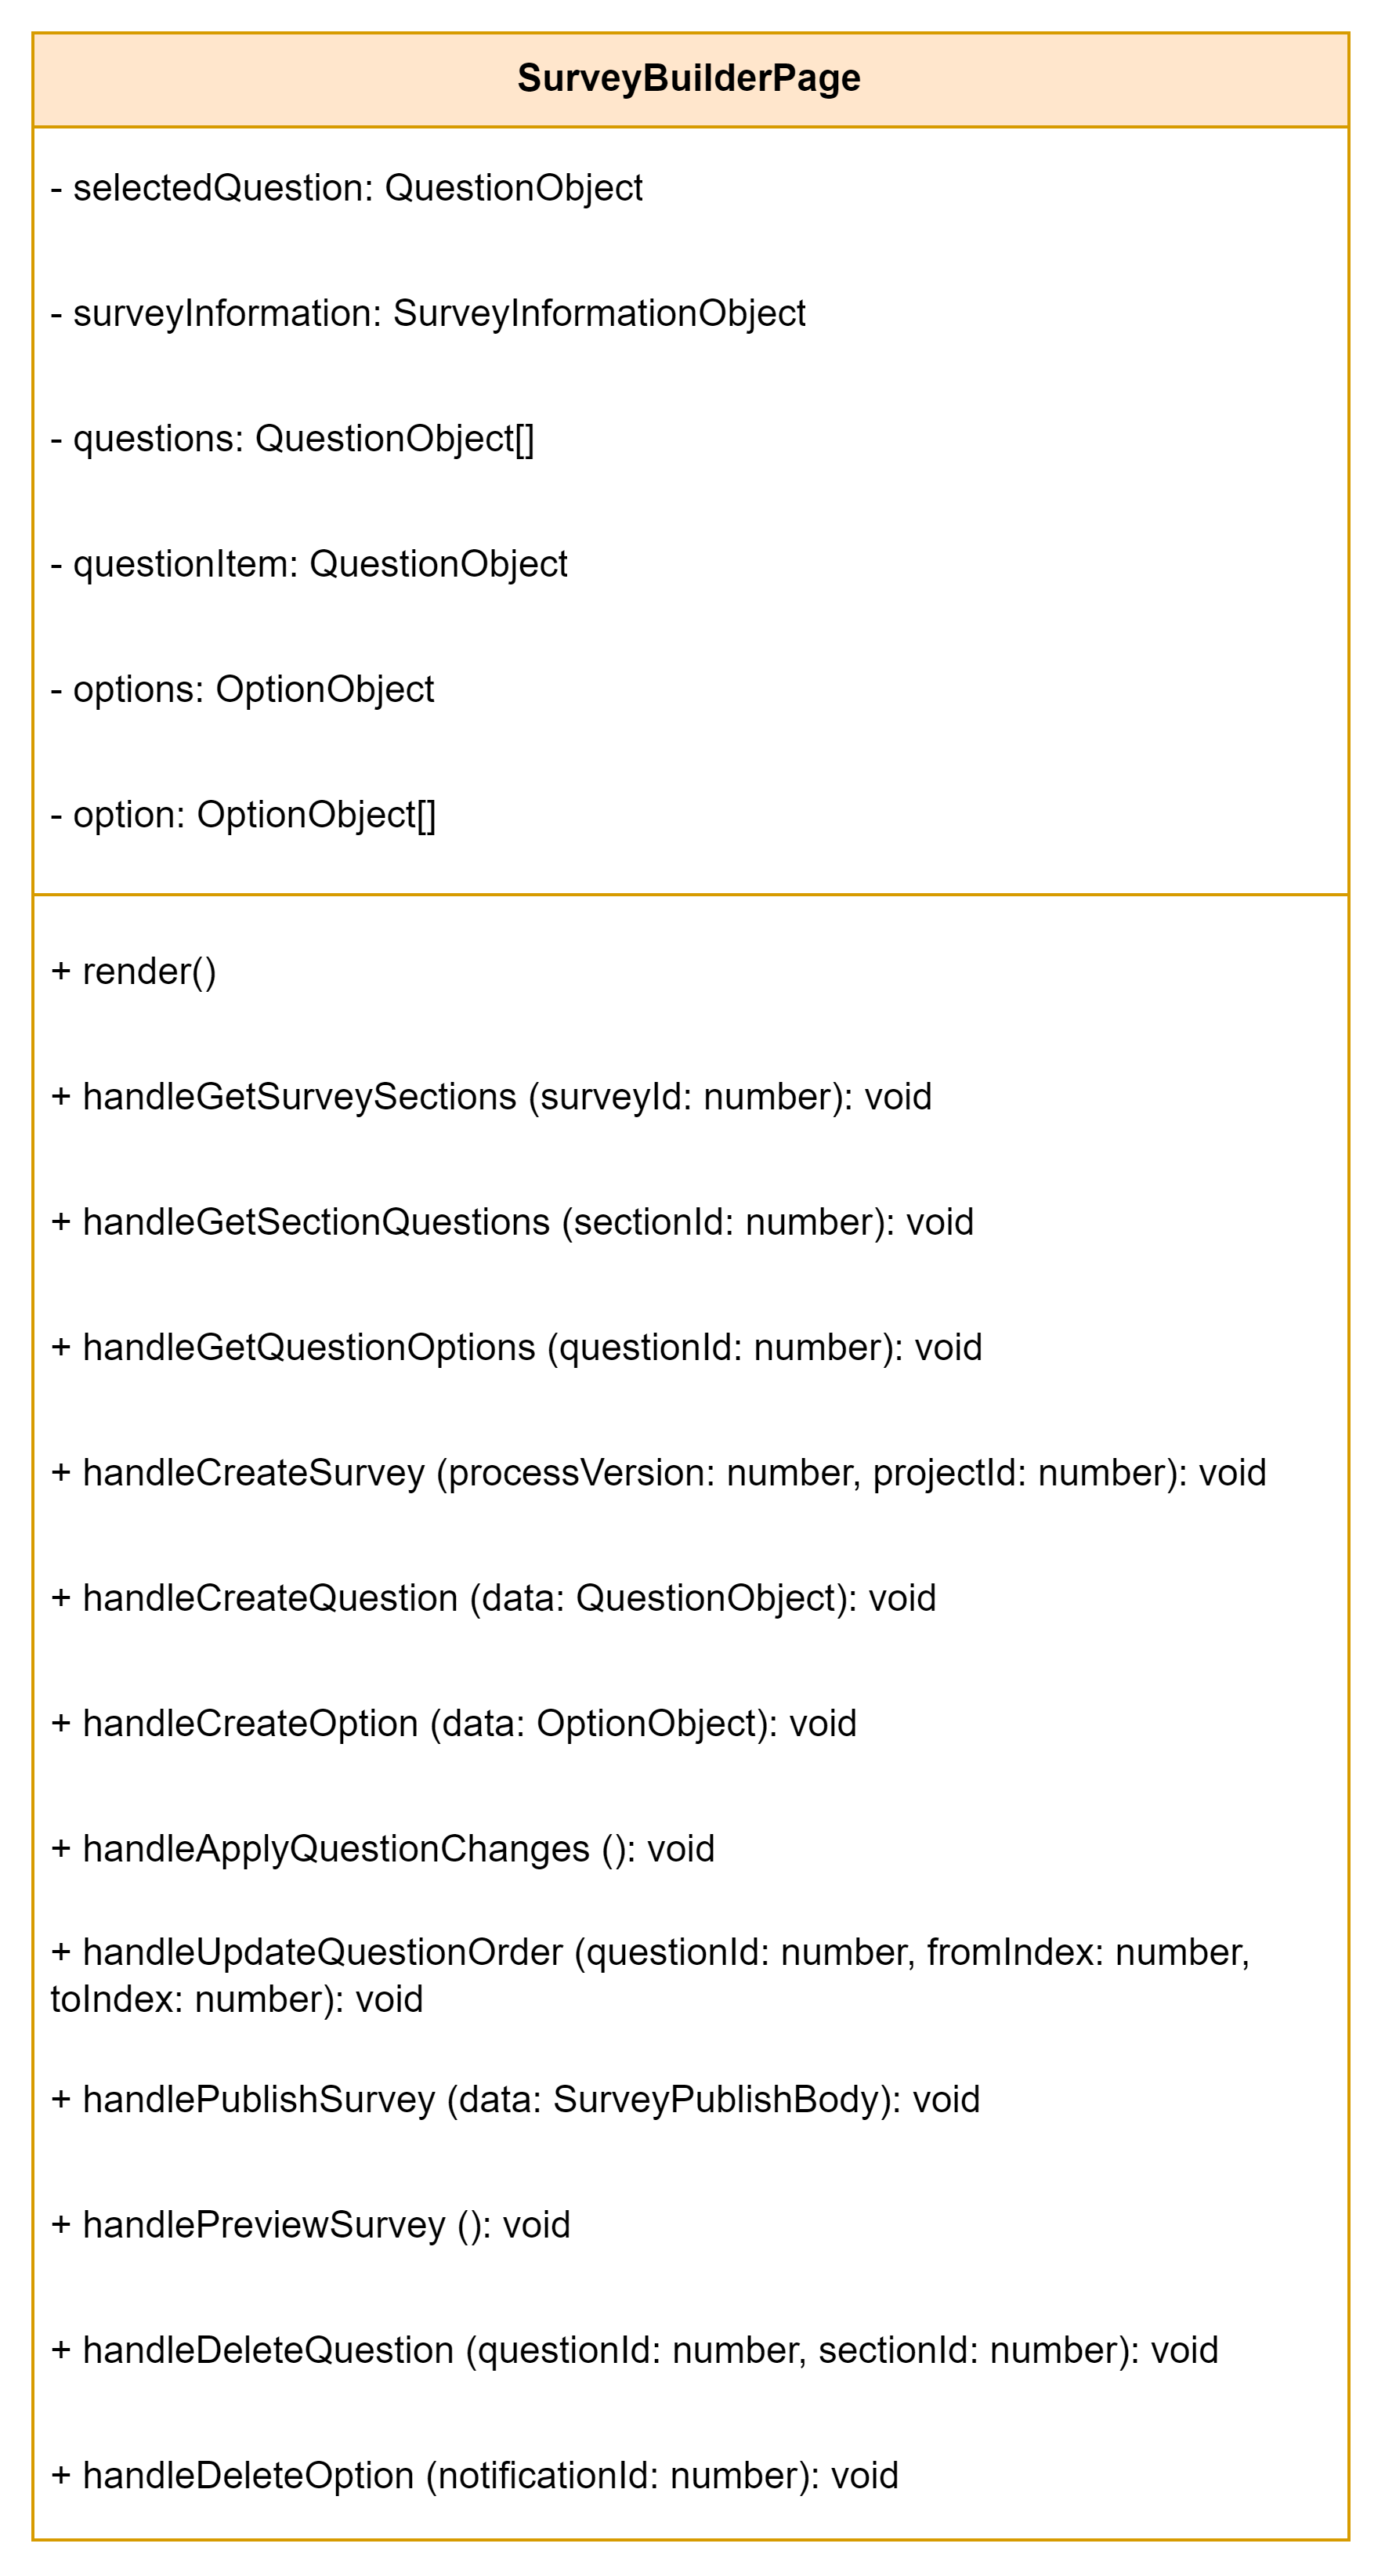
\includegraphics[ width = 0.4\linewidth]{Content/Phân tích và thiết kế hệ thống/documents/Sơ đồ lớp/images/Presentation layer/surveyBuilderPage.png}
    \vspace{0.5cm}
    \caption{Class SurveyBuilderPage trong Presentation layer}
    \label{fig:Class SurveyBuilderPage trong Presentation layer}
\end{figure}
Giao diện chỉnh sửa khảo sát sẽ bao gồm 2 phần là khu vực để hiển thị danh sách những câu hỏi có trong khảo sát và khu vực để chỉnh sửa thuộc tính của câu hỏi, bao gồm nội dung câu hỏi, các lựa chọn (nếu câu hỏi thuộc loại multiple choice), cài đặt yêu cầu người dùng bắt buộc phải trả lời câu hỏi hay không, cài đặt trọng số của câu hỏi. Ngoài ra, người dùng có thể thay đổi vị trí của hỏi trong khảo sát thông qua thao tác kéo thả.

\begin{figure}[H]
    \centering
    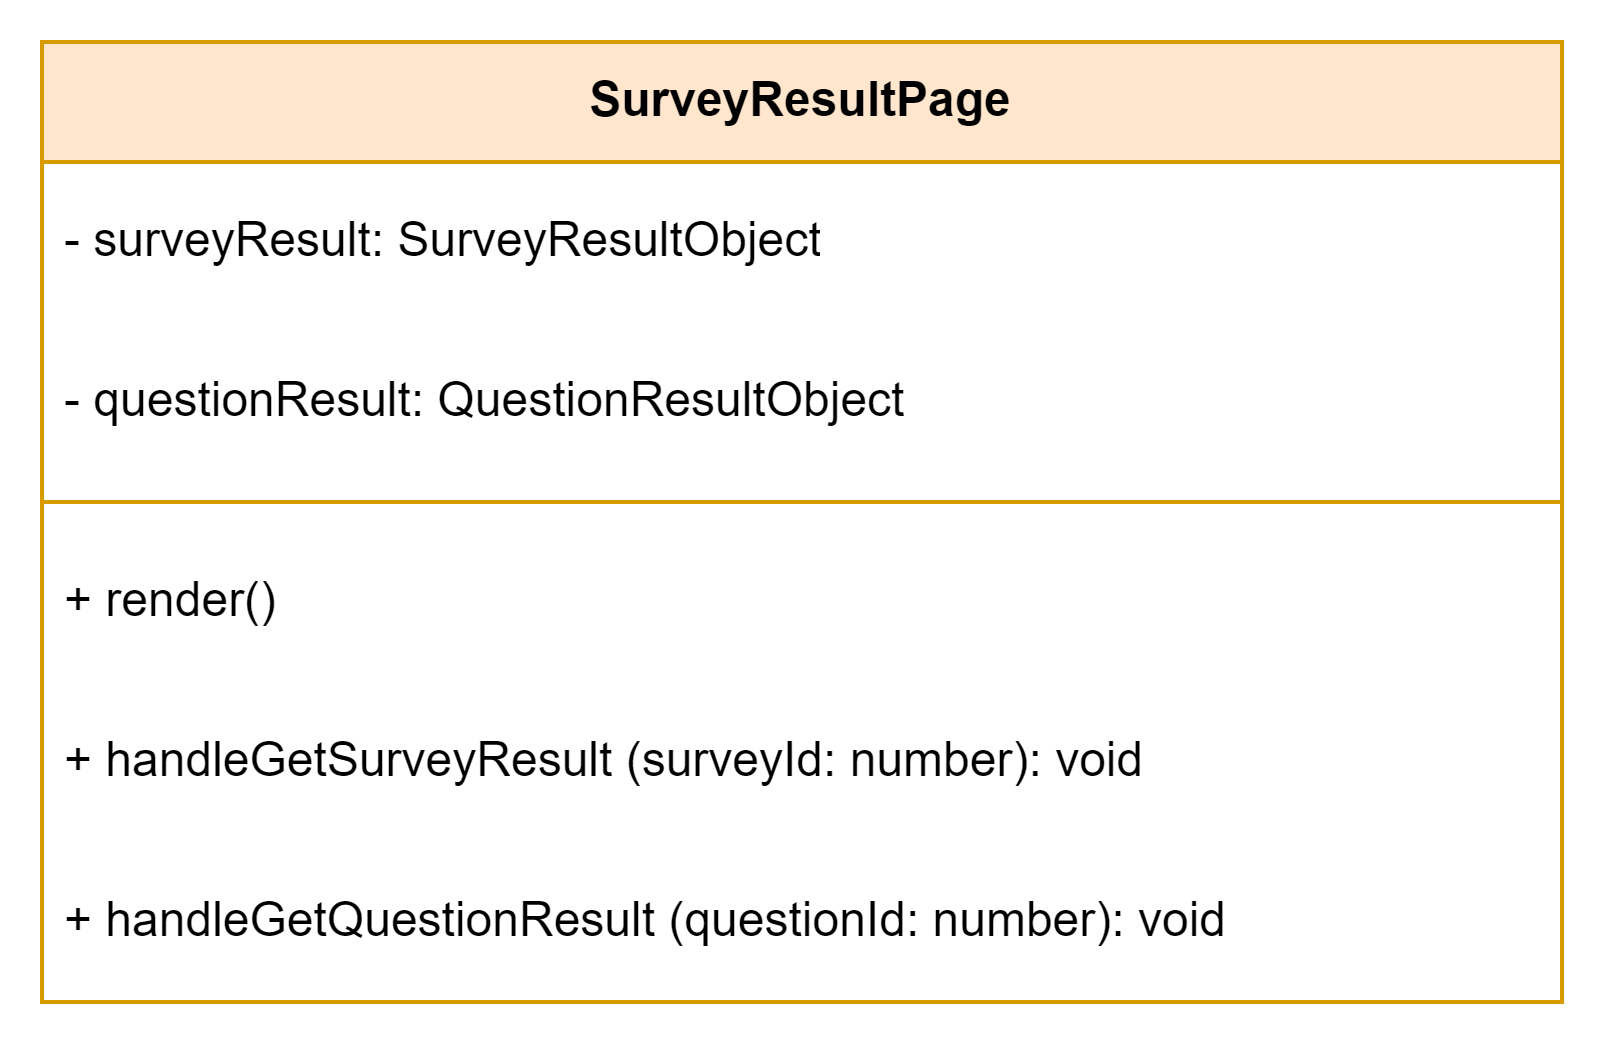
\includegraphics[ width = 0.5\linewidth]{Content/Phân tích và thiết kế hệ thống/documents/Sơ đồ lớp/images/Presentation layer/surveyResultPage.png}
    \vspace{0.5cm}
    \caption{Class SurveyResultPage trong Presentation layer}
    \label{fig:Class SurveyResultPage trong Presentation layer}
\end{figure}
Giao diện hiển thị kết quả khảo sát sẽ hiển thị kết quả tổng hợp của khảo sát và kết quả của từng câu hỏi. Kết quả sẽ được biểu diễn thông qua biểu đồ cột và tròn tương ứng với loại câu hỏi.

\begin{figure}[H]
    \centering
    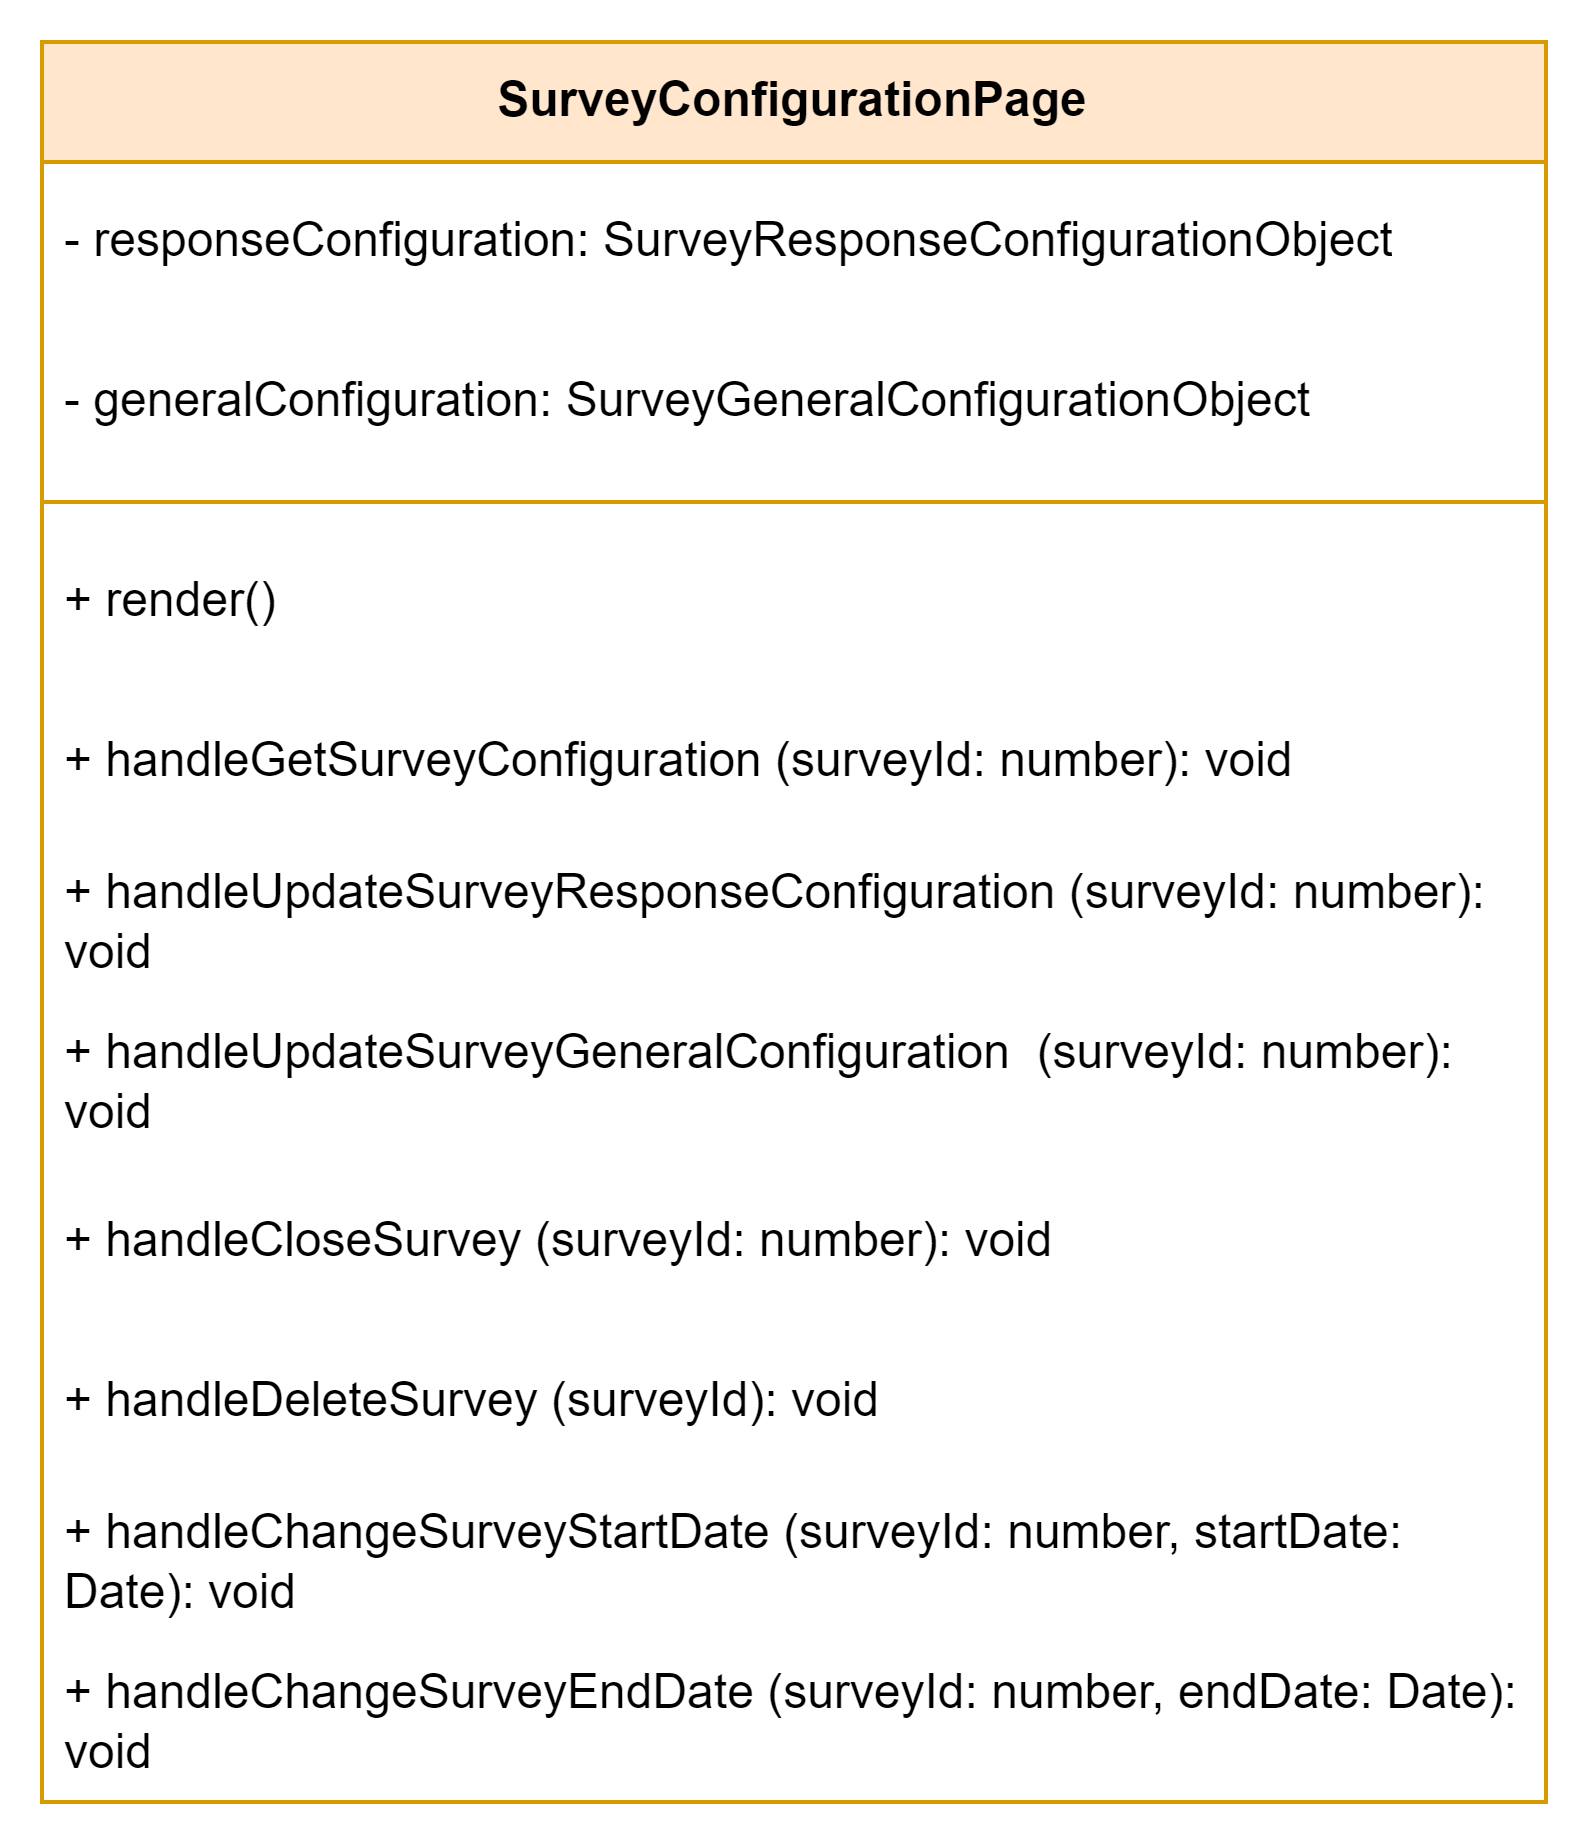
\includegraphics[ width = 0.4\linewidth]{Content/Phân tích và thiết kế hệ thống/documents/Sơ đồ lớp/images/Presentation layer/surveyConfigurationPage.png}
    \vspace{0.5cm}
    \caption{Class SurveyConfigurationPage trong Presentation layer}
    \label{fig:Class SurveyConfigurationPage trong Presentation layer}
\end{figure}
Giao diện chỉnh sửa cấu hình của khảo sát cho phép người dùng cài đặt thời gian công bố/đóng khảo sát, cũng như cài đặt cho phép người dùng thực hiện khảo sát nhiều lần. Ngoài ra, cũng có thể chỉnh sửa tên và mô tả của khảo sát tại đây.

\begin{figure}[H]
    \centering
    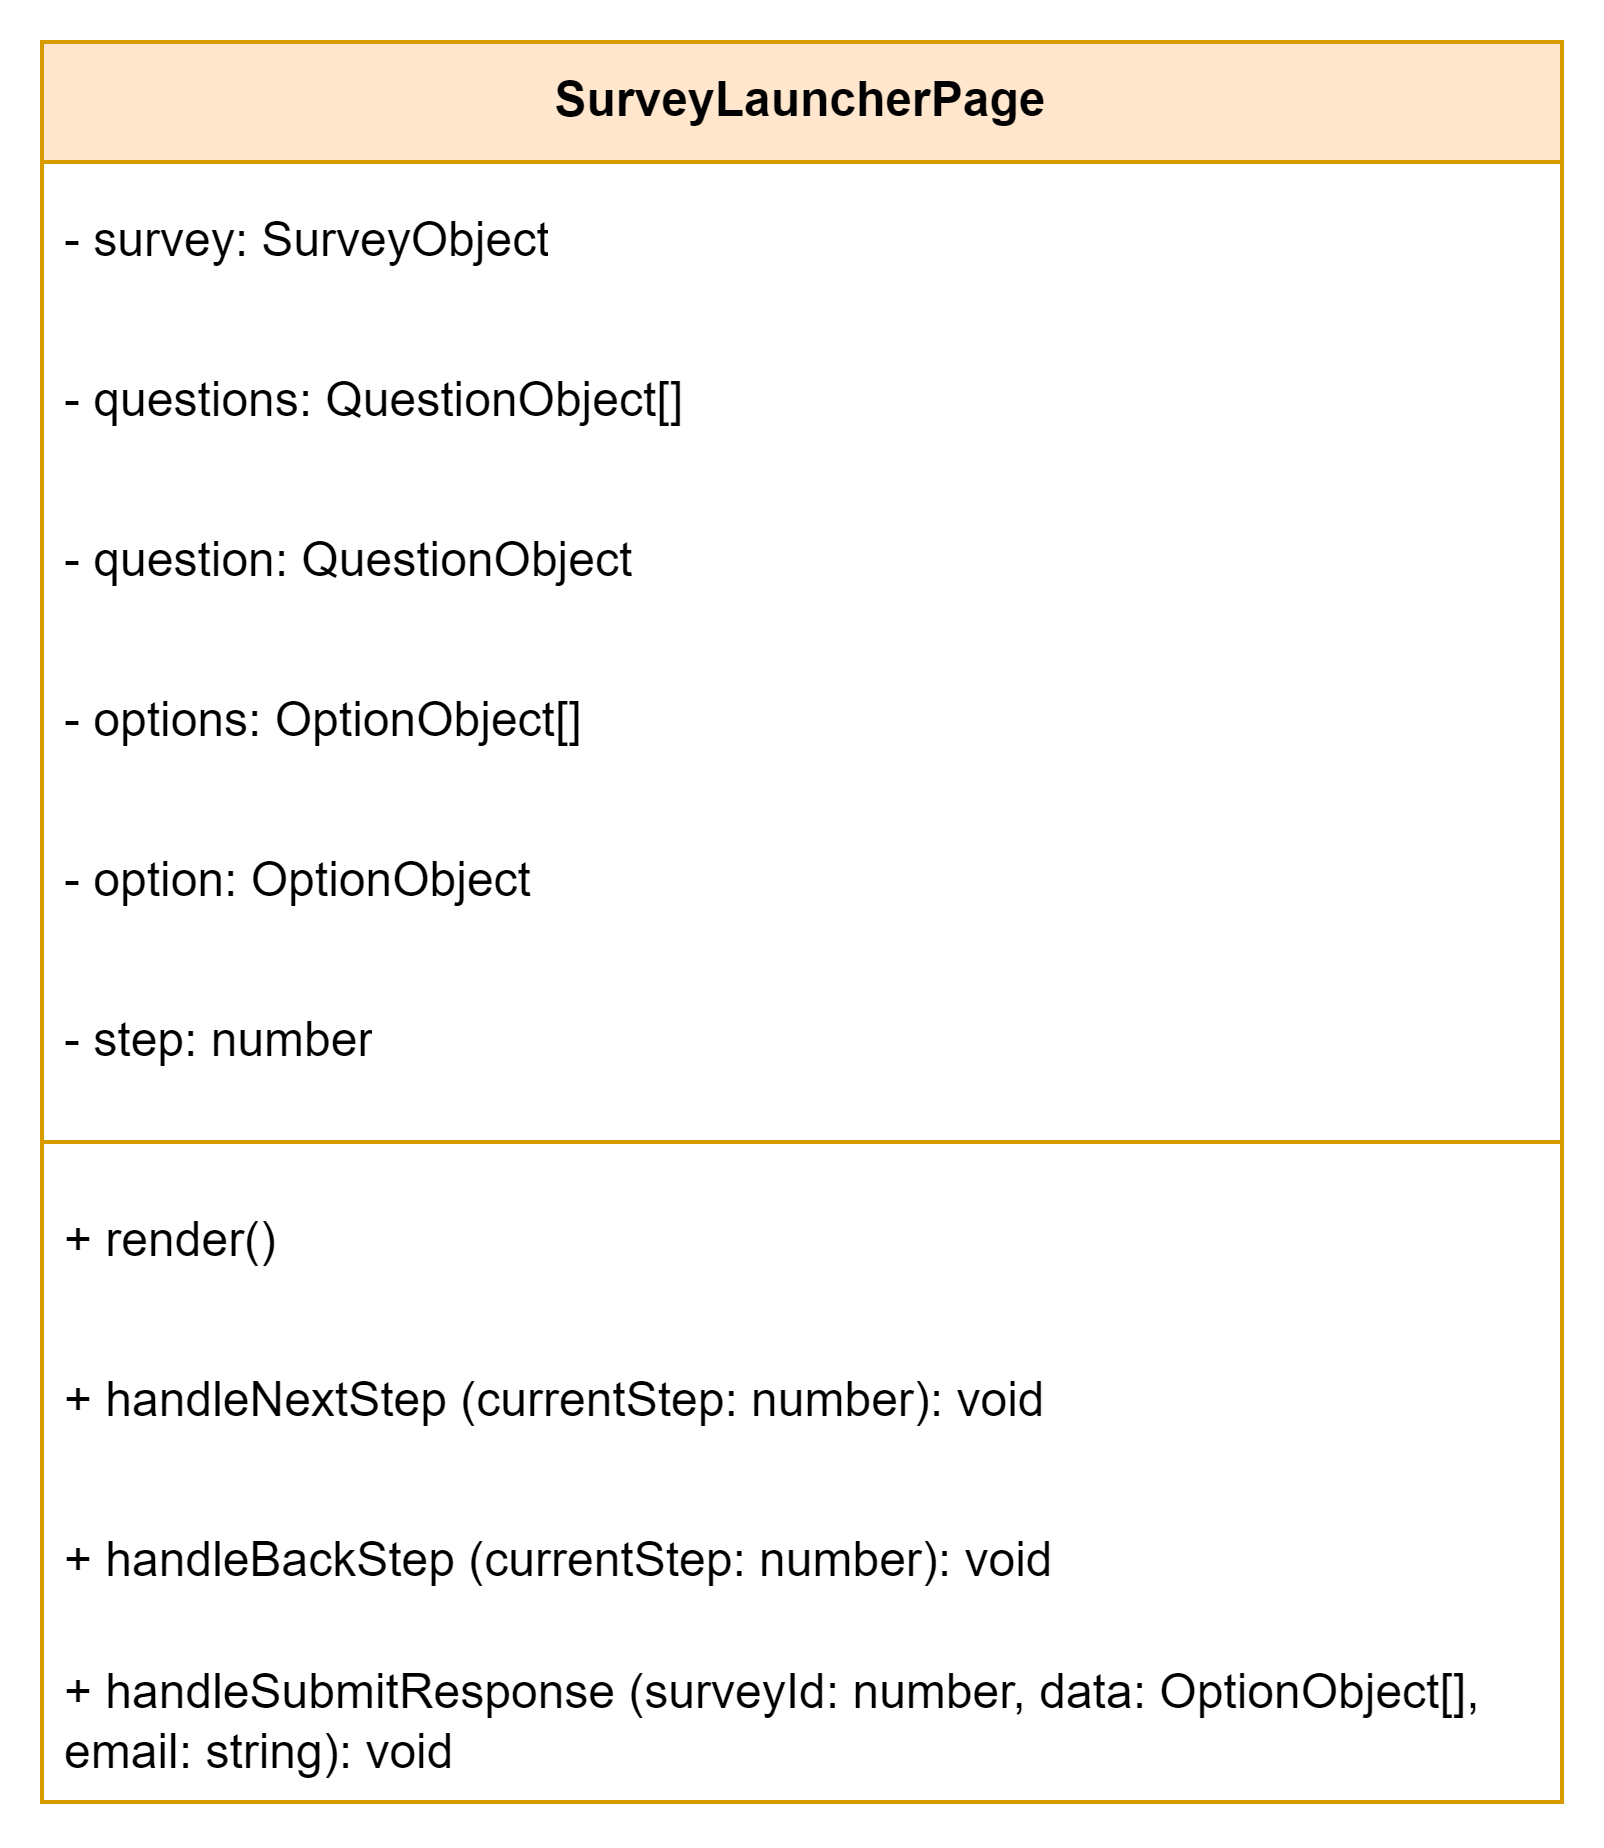
\includegraphics[ width = 0.4\linewidth]{Content/Phân tích và thiết kế hệ thống/documents/Sơ đồ lớp/images/Presentation layer/surveyLauncherPage.png}
    \vspace{0.5cm}
    \caption{Class SurveyLauncherPage trong Presentation layer}
    \label{fig:Class SurveyLauncherPage trong Presentation layer}
\end{figure}
Giao diện này cho phép người dùng gửi phản hồi cho khảo sát, người dùng có thể truy cập vào khảo sát thông qua đường dẫn được người tạo khảo sát gửi trực tiếp hoặc thông qua hòm thư điện tử. Khảo sát sẽ chia thành nhiều phần khác nhau, người dùng có thể chọn đến phần tiếp theo hoặc quay trở lại phần trước đó để chỉnh sửa phản hồi của mình. Để gửi khảo sát người dùng cần cung cấp email và tên người dùng để nhận kết quả sau khi khảo sát tổng kết kết quả.